% BACKGROUND & RELATED WORK
%
% !TEX root = ../thesis-main.tex
%
\chapter{Background and related work}
\label{chap:background}

%\cleanchapterquote{You can’t do better design with a computer, but you can speed up your work enormously.}{Wim Crouwel}{(Graphic designer and typographer)}


\section{Pronunciation in foreign language education}
\label{sec:bkgd:pron}

\citep{Derwing2005,Dlaska2013,Hirschfeld2007,Mehlhorn2005}

In the foreign language classroom, less focus has traditionally been placed on pronunciation than on other aspects of language education, such as grammar and vocabulary \citep{Neri2002}.

However, even when pronunciation is taught in the classroom, a number of factors may limit the effectiveness of that training \citep{Neri2002}. First of all, many teachers lack the training in phonetics and phonology to provide helpful feedback to students and correct their articulation \TODO{citation}. Secondly, high student-to-teacher ratios may prevent teachers from giving adequate attention and feedback to individual students, and limit the amount of time each student can practice speaking. Furthermore, anxiety about speaking the L2 in front of their peers may make students less willing to practice speaking, and less able to absorb corrective feedback.

%CAPT may also be perceived by the learner as a lower-stakes, more comfortable environment than the classroom, where they may feel too intimidated to practice speaking in the L2.


\section{Computer-Assisted Pronunciation Training} %TODO Teaching,Training?
\label{sec:bkgd:capt}

	The value of speech technologies in foreign-language teaching has been well demonstrated in recent decades \citep{Neri2002,Eskenazi2009,Delmonte2011,Witt2012}. Computer-Assisted Pronunciation Training (CAPT) has emerged as one important educational application of speech technology. Indeed, as \textcite{Neri2002} point out, CAPT stands to overcome the hurdles of teacher-led pronunciation training described in the previous section.
	
	The viability of CAPT has been demonstrated by a variety of systems and tools that have been developed in both academic and commercial contexts. Some tools focus on overall assessment of pronunciation or fluency, while others focus on the detection and correction of individual pronunciation errors \citep{Eskenazi2009}; the tool developed in this work will fall into the latter category. In error-focused systems, a distinction has typically been drawn between phonemic errors, e.g. the substitution, insertion, or deletion of a segmental speech sound, and prosodic errors, such as those related to stress/accent, intonation, or rhythm \citep{Witt2012}. As we saw in the previous section, prosodic errors have a larger impact on intelligibility, and will be the focus of this work (see \cref{sec:bkgd:targeting} below). With this in mind, a few CAPT systems relevant to this thesis are discussed below; overviews and comparisons of these and many other systems are given by \textcite{Neri2002,Eskenazi2009,Delmonte2011,Witt2012}.  
	
	
	
%	\subsection{Pronunciation in foreign language education}
%	\label{sec:capt:l2ed}
%	
%	The difficulties posed by including pronunciation in the foreign language classroom curriculum will be discussed in this section, leading to the conclusion that CAPT can help make pronunciation training more accessible by overcoming some of these difficulties (e.g. teacher-to-student ratio). Relevant findings from a variety of works on pronunciation teaching in the classroom will be presented .

%	\subsection{Computer-based and intelligent tutoring systems?} 
%	\label{sec:capt:its}
%	%TODO is this section necessary?
%	
%	This section would serve as a domain-independent overview of CBT and ITS, and the advantages such systems can bring when deployed in schools or used individually.
	
%TODO replace
%	\subsection{Prosody in existing CAPT systems}
%	\label{sec:capt:systems}
	
	%This section will describe a selection of related CAPT systems and tools, and how these tools have analyzed and offered feedback on speech prosody.
	
	Both the diagnosis and feedback modules of the CAPT tool developed in this work will build to a great extent on previous work by researchers in the speech group at LORIA in Nancy, many of whom are also involved in the IFCASL project (see \cref{sec:intro:ifcasl}). Their work has, on the one hand, investigated the task of automatically recognizing and segmenting learners' speech, and determining how this possibly incorrect automatic segmentation can be effectively utilized in the context of pronunciation tutoring, particularly at the prosodic level \citep{Mesbahi2011,Orosanu2012}; see \cref{chap:diagnosis} for a discussion of how this thesis will build upon that work. Additionally, the group has developed the \textit{Snoori} suite of software, including the PC-based WinSnoori and its partial Java port, Jsnoori \citep{Parole2013}.  %TODO properly cite Jsnoori/WinSnoori?
These programs take as input a learner utterance, a native reference utterance, and segmentations of each, perform an acoustic comparison of the two utterances, and deliver feedback on the learner's speech in the form of e.g. annotated displays of the speech signal and spectrogram of each. Moreover, auditory feedback can be delivered thanks to the capability of resynthesizing the learner's utterance to match the pitch contour and timing of the reference, without modifying the voice quality of the utterance, such that the learner can hear the ``correct'' pronunciation in their own voice. The utility of such software, and especially this resynthesized feedback, for pronunciation teaching has been explored by \textcite{Bonneau2011}, who used it to assess and deliver feedback on lexical stress in L1 French speakers' pronunciation of English words. %TODO more about the Bonneau paper?
As described later in this paper, the proposed thesis will, on the one hand, build on the error detection and diagnosis functionality of Jsnoori (see \cref{chap:diagnosis}), as well as leverage its feedback generation capabilities to deliver a more diverse, and potentially more effective, range of feedback types (see \cref{chap:feedback}). 
	
	% \citep{Bonneau2011,Fohr1996,Fohr2012,Mesbahi2011,Orosanu2012}. The Jsnoori/WinSnoori software \citep{Parole2013}
%which this group has developed will be instrumental in the construction of the CAPT tool. 
	
	This work will also draw from research conducted at Carnegie Mellon University in Pittsburgh, particularly in the context of the Fluency pronunciation training system \citep{Eskenazi1998,Eskenazi2000,Probst2002} and the LISTEN project and its Reading Tutor \citep{%
	Duong2011,
	Mostow2012,
	Mostow1999,
	Sitaram2011,
	%Weber2010
	}. 
	
	In the Fluency CAPT system, particular emphasis is placed on
%prosody and 
user-adaptivity, corrective articulatory feedback, and the integration of perceptual training (e.g. listening exercises) \citep{Eskenazi2000}. As with the work at LORIA described above, the Fluency system evaluates learners' speech via comparison with that of a native reference speaker, and \textcite{Probst2002} found that selecting a ``golden speaker'' whose voice closely matched the learner's improved learning gains. Fluency also implements an error-catching step to reject utterances which do not match the expected text \citep{Eskenazi2000}, in the same vein as that of \textcite{Mesbahi2011,Orosanu2012}. \textcite{Eskenazi2007} report that Fluency's commercial spin-off, NativeAccent\textsuperscript{TM}, has been shown to help real-world users significantly improve their pronunciation skills.
	%In an early version of Fluency, an utterance is elicited from the learner using a targeted question, constraining the learner's response such that a speech recognizer can perform forced alignment on the utterance, while at the same time giving the learner the impression that they have decided what to say (as opposed to simply reading a given sentence out loud).
	
	The Reading Tutor is not strictly a CAPT tool, as it is designed to help children develop their reading fluency in their native language. However, as it analyzes the prosody of children's read speech to measure reading fluency, and offers feedback on this prosody, it is nevertheless very relevant to CAPT and thus this thesis. 
	%Indeed, the potential for such a tool, and its underlying technologies, to enhance foreign-language education has already been demonstrated by \textcite{Weber2010}, who deployed the Reading Tutor in English as a second language classes in India with encouraging initial results. 
	In the Reading Tutor, the child's read speech is automatically segmented and compared either to a reference utterance by an adult reader, analogous to the native speaker reference in many CAPT systems, or to a generalized model of adult prosody \citep{Duong2011}. Analysis of the pitch and intensity contours of the utterances, as well as the duration of words/syllables and the spaces between them, results in an assessment of the child's overall fluency as well as identification of words which have been pronounced (in)correctly, and feedback is delivered visually in real time by revealing the text of each word as it is spoken, with properties such as the position, color, and font size of each word reflecting various aspects of the reader's prosody \citep{Sitaram2011}. This thesis will incorporate ideas and techniques from the Reading Tutor, in both its diagnosis (see \cref{chap:diagnosis}) and feedback (see \cref{chap:feedback}) modules. %TODO reword that
	
	The vast majority of CAPT systems which analyze learners' speech at the prosodic level have been developed with English as the target L2, though there are some notable exceptions.
	\TODO{Delmonte's SLIM?}, \TODO{VILLE Swedish thing}, as well as \TODO{Jilke's German intonation thing}. \TODO{anything else in German}?
	
	%Other systems mentioned by \textcite{Eskenazi2009,Delmonte2011,Witt2012} may also be briefly described, including tools developed at KTH \citep{Hincks2002,Hincks2009} to teach English prosody.
	
	
% Alternative organization:
 \section{Lexical stress}
 \label{sec:bkgd:stress}
		%TODO check this section for inaccuracies
		When there is a typological difference between some segmental or prosodic feature(s) of a language learner's L1 compared to the target L2, there is a particular need for pronunciation training to bridge this gap. In the case of the French-German language pair, the prosodic realization of lexical stress is one feature which marks a striking difference between the languages.
		
			Lexical stress is the phenomenon of how syllables are accentuated within a word  \citep{Cutler2005}. This relates not to the segmental characteristics of a syllable, i.e. the speech sounds it contains, but rather to its (relative) suprasegmental properties, namely: %TODO need citation here?
			\begin{itemize}
			\item duration, which equates on the perceptual level to timing;
			\item fundamental frequency (F0), which corresponds to perceived pitch; and
			\item intensity (energy or amplitude), which perceptually equates to loudness.
			\end{itemize}

%TODO more text here? or move text from German vs French section here?
		
		%\subsection{German vs. French}
		%\label{sec:stress:GvF}
		
					As \textcite{Cutler2005} points out, different languages make use of this suprasegmental information in different ways.
			In what are termed free- or variable-stress languages, such as German, Spanish, and English, it is not always possible to predict which syllable in a word will carry the stress, and therefore knowing a word requires, in part, knowing its stress pattern. This allows stress to serve a contrastive function in these languages, such that two words may share exactly the same sequence of phones and nevertheless be distinguished exclusively by their stress pattern, as is the case with \textit{UMfahren} (to drive around) and \textit{umFAHRen} (to run over with a car) in German. %TODO better example of minimal pair
Because stress carries meaning thus, native speakers of such languages are sensitive to stress patterns, and readily able to perceive differences in stress. %TODO wording?

			However, in the so-called fixed-stress languages, stress is completely predictable, as it always falls on a certain position in the word; in Czech and Hungarian, for example, stress always falls on the word-initial syllable. Therefore, lexical stress may not be as crucial to the knowledge of a word in these languages as in the free-stress languages. Furthermore, although lexical stress is realized in these languages, the distinction between stressed and unstressed syllables may be weaker than in free-stress languages. French has often been placed into this category of fixed-stress languages, although it may be more properly considered a language without lexical stress, insofar as there is no systematic way in which speakers distinguish a certain syllable from others in the word, aside from the fact that French exhibits phrasal accent, i.e. lengthening of the final syllable in each prosodic group or phrase \citep{Dupoux2008}. %TODO other references?			
			
		Therefore, native speakers of French may lack the sensitivity to stress patterns possessed by native speakers of German. Indeed, this has been borne out by research by \citeauthor{Dupoux2008} \citep{Dupoux2001,Dupoux2008}, which demonstrated that native French speakers were ``deaf'' to differences in stress patterns, such that they have great difficulty discriminating between Spanish words which contrast only at the level of stress. This difficulty should also exist for French speakers when they are presented with German words in which the stress pattern is crucial to the word's meaning, as in the minimal pair above.
		
%		\subsection{Lexical stress in foreign language teaching?}
%		\label{sec:stress:l2ed}
%		
%		This section may be merged into \cref{sec:capt:l2ed} above.
%		
%		\citep{Hirschfeld2007}
		
		
 \section{Targeting lexical stress errors in CAPT}
 \label{sec:bkgd:targeting}
 	Learners of a foreign language typically make a wide variety of pronunciation errors, at both the segmental level (e.g. errors in producing certain individual phones of the target language) and the prosodic level (e.g. errors in the speaker's intonation contour or the duration of certain syllables or words). As it is not possible to address all of these in an automated system, one of the first aims of this work is to identify a single type of error which is well suited to being addressed via a CAPT system targeting French L1 learners of German as the L2. 
	
	To guide this selection, we may consider %TODO wording
a set of three criteria that such an error must meet; similar criteria are proposed by \textcite{Cucchiarini2009}.
%As illustrated in \cref{fig:errors}, t %TODO replace reference after proposal
The best error to target with the CAPT system will fulfill all of these criteria, rather than only one or two of the three. The criteria are:

\begin{enumerate}

\item The error must be produced with a some degree of frequency by French L1 speakers in their production of L2 German, as it would be a misuse of resources to design a system which addresses an error that is seldom made by learners \citep{Neri2002}.

\item The error must have a significant impact on the perceived intelligibility of the learner's speech; as the ultimate goal of the system is to help learners communicate more effectively in the L2, an error which is commonly made but nevertheless does not impede understanding of the learner's L2 speech, and thus does not hinder communication in the L2, is not an ideal target. 
It should be noted here that intelligibility, and not lack of a ``foreign accent'', is generally considered to be the most important goal of pronunciation training \citep{Neri2002,Witt2012}.

\item In order for the CAPT system to provide any meaningful diagnosis and feedback, the error must lend itself to reasonably accurate and reliable  detection through automatic processing. 

\end{enumerate}

	
%TODO replace figure after proposal
%		%\begin{center}
%		\begin{figure}[htb]
%			\centering
%			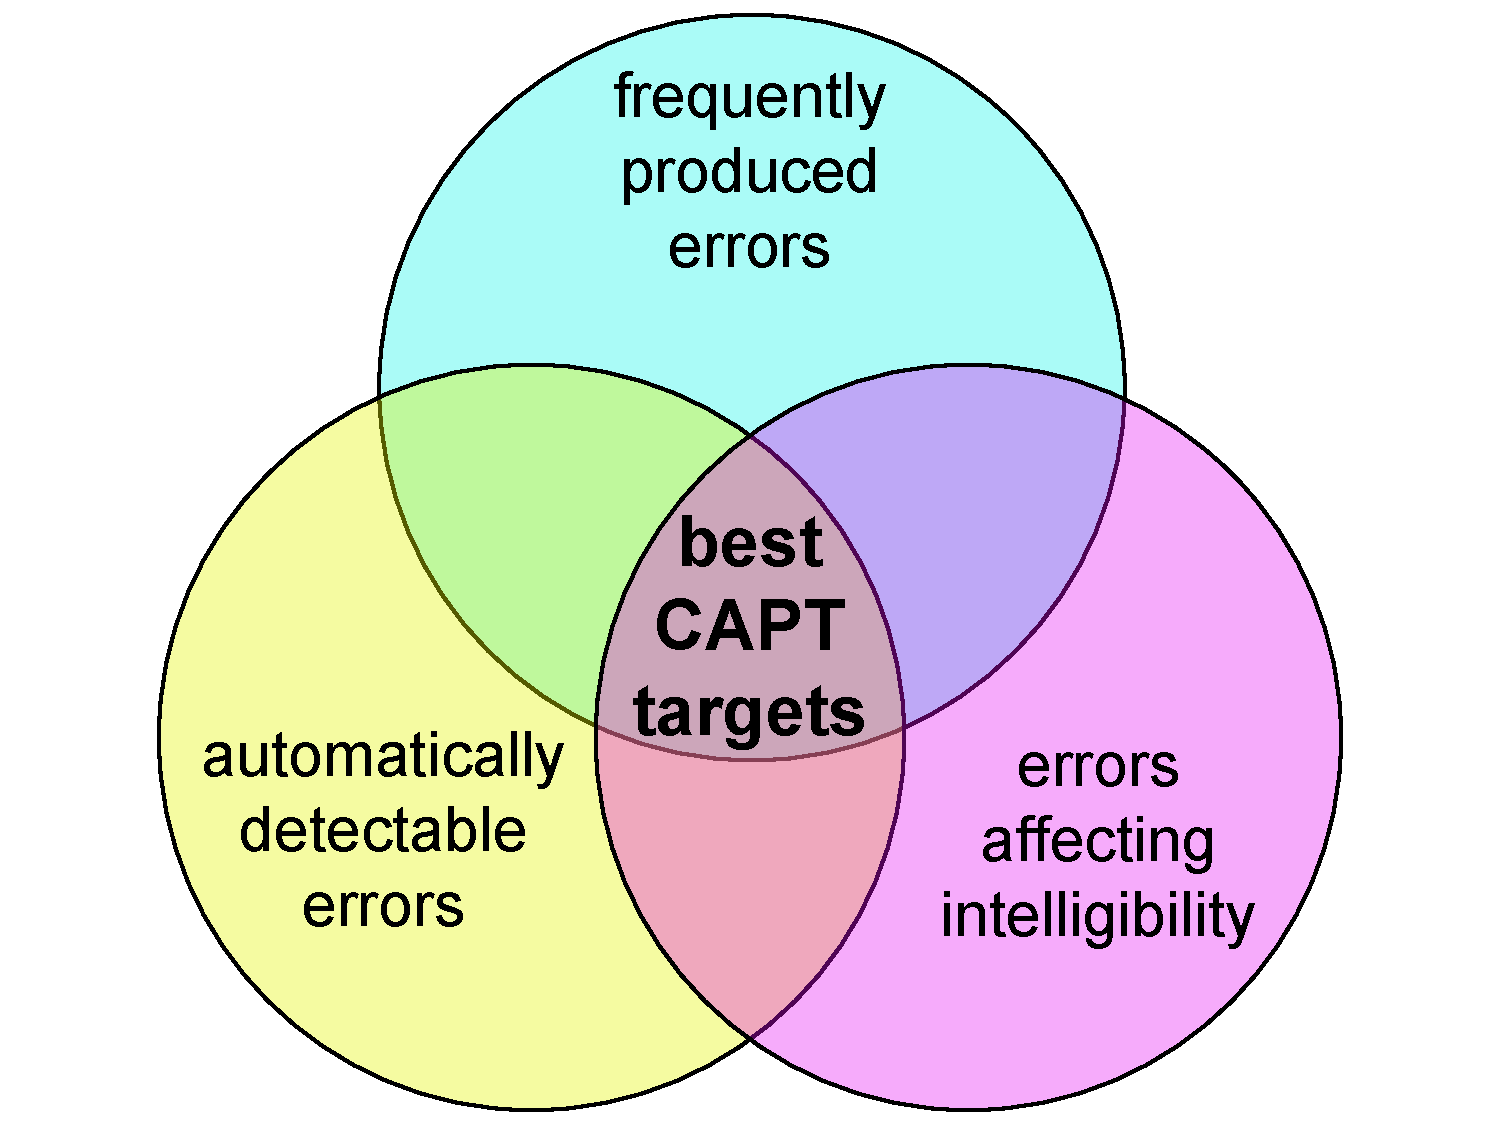
\includegraphics[width=.7\textwidth]{../img/error-venn}
%			\caption{Criteria for selecting errors to target in a CAPT system.}
%			\label{fig:errors}
%		\end{figure}
%		%\end{center}
	
	This thesis proposes that lexical stress errors are a strong candidate for treatment via CAPT, insofar as this type of error meets the above criteria. 
Lexical stress errors are frequently produced by L1 French speakers when learning a free-stress L2 \TODO{citation}.
	
	Lexical stress errors will therefore be the focus of the prototype system which will be developed.
	 
	 %TODO take the below out?
	 %For example, vowel quality errors (e.g. an L1 French speaker producing a German /\textipa{@}/ as [\textipa{\oe}]) may occur frequently in the L2 speech and may be relatively easy to detect automatically, but may not have a great impact on the intelligibility of the L2 German speech. On the other hand, equally frequent vowel quantity errors (e.g. the L1 French speaker producing a German long /\textipa{e:}/ as [\textipa{e}]) may have a greater impact on intelligibility in some cases, but may be more difficult to reliably identify automatically.
	
%TODO remove
	%Analysis of the typical and expected errors described in \cref{sec:CAPT4FG:comparison} in terms of these criteria reveals that lexical stress errors are a strong candidate for treatment via CAPT, and will therefore be the focus of the prototype CAPT system described in this thesis. The remainder of this section justifies the selection of this type of error by describing how it fulfills the aforementioned criteria as well or better than any other error type.
	

%TODO replace
%		\subsection{Impact on intelligibility}
%		\label{sec:targeting:intelligibility}

	Research on the impact of various types of pronunciation errors (e.g. \cite{Hirschfeld1994,%
	%Raux2002	%TODO include?
	}) has generally shown that errors related to prosody have a larger impact on the perceived intelligibility of the L2 speaker than errors on the segmental level \citep{Witt2012}.

		\citep{Warren2009}
		
		\citep{Magen1998}
		
		Furthermore, lexical stress not only impacts intelligibility on the prosodic level, but may also affect perception of segmental errors in the L2 learner's speech; for example, segmental errors occurring in stressed syllables are more noticeable than those in unstressed syllables \citep{Cutler2005}.
		
		``Prosody errrors in particular tend to contribute to any perceived accent more so than individual phoneme mispronunciations.'' \citep[p.~6]{Witt2012}
				
%TODO replace	
%		\subsection{Frequency of production}
%		\label{sec:targeting:frequency}
		\citep{Cutler2005}
		
		\citep{Peperkamp2002, Dupoux2001, Dupoux2008}
		
		 
		
%TODO replace
%		\subsection{Feasibility of automatic detection}
%		\label{sec:targeting:autodetect}

		Detecting syllable- or word-level errors may be more feasible than detecting phone-level errors: ``One additional challenge in pronunciation error detection is that a phoneme represents the smallest possible unit compared to the syllable, word, and sentence level. The shorter the unit, the higher will be the variability in the judgment of the pronunciation quality.'' \citep[p.~2]{Witt2012}

		\citep{ISADEPT, Delmonte2011}
		
		\citep{Bonneau2011}
		
		\citep{Shahin2012a,Kim2011}
		
% \section or \subsection{Other related work on lexical stress in CAPT}

% Old section:
%\section{Towards CAPT for French learners of German}
%\label{sec:CAPT4FG}
	
% Alternative organization:
%	\subsection{Targeting errors in CAPT}
%	\subsection{Lexical stress in French and German}
%	\subsection{Targeting lexical stress errors}

% Old organization:
%	\subsection{Phonetic and phonological comparison}
%	\label{sec:CAPT4FG:comparison}
%		\subsubsection{Segments}
%		\subsubsection{Prosody}
%
%			\paragraph{Lexical stress}
%			
%		\subsubsection{Other factors}
%		
%	\subsection{Targeting lexical stress errors}
%	\label{sec:CAPT4FG:targeting}
%
%		\subsubsection{Frequency of production}
%		
%		\subsubsection{Impact on intelligibility}
%		
%		\subsubsection{Feasibility of automatic detection}
%		

%TODO replace
%\section{Summary}
%\label{sec:bkgd:summary}